\documentclass[11pt]{article}
\usepackage[utf8]{inputenc}

\usepackage{url}
\usepackage{verbatim}
\usepackage{enumitem}
\usepackage{tcolorbox}
\usepackage{xcolor-material}
\usepackage{tabularx}

\usepackage{tabulary}
\usepackage{booktabs}

\usepackage[british]{babel}

\title{Advanced SE -- Envisioning}
\author{\begin{minipage}{0.655\linewidth}
\textbf{E}leonora Pura, \url{eleonora.pura@uzh.ch}, 17-732-678\\
\textbf{N}icolas Kohler, \url{nicolasfazli.kohler@uzh.ch}, 16-712-887\\
\textbf{O}liver Kamer, \url{oliver.kamer@uzh.ch}, 16-921-009\\
\textbf{C}hristian Omlin, \url{christian.omlin@uzh.ch}, 14-936-165\\
\textbf{A}lain Küng, \url{alain.kueng@uzh.ch}, 18-717-017\\
\end{minipage}}

\usepackage[margin=1in, includefoot]{geometry}
\usepackage{parskip}

\usepackage{tikz}
\usepackage{aeguill}

\begin{document}

\maketitle

\setcounter{tocdepth}{1} %only sections in table of contents

\tableofcontents

\section{Project Context}
Many code-sharing repositories already offer some way of highlighting written code. However, we believe that there is further room for improvement. Thus, we aim to improve upon currently existing syntax highlighting software, by applying and training an existing neural network. For this, we plan to offer an easy-to-use, microservice-based solution to help color-highlight source code files. The machine learning algorithm continuously improves its accuracy upon receiving more source code. The advantage of the deep learning model is that it will also be useful for incorrect or incomplete language derivations, in contrast to many other solutions today. As part of this project we plan to support the common languages Python, Java, and Kotlin. However, our goal is to design the code base in such a way that additional programming languages can be added in the future with little effort.

\subsection{Stakeholders}
In the following we will group the identified stakeholders into four groups: primary, secondary, tertiary and facilitating stakeholders. The primary group entails stakeholders who use the system directly, while the secondary group is concerned about stakeholders who provide input or receive output from the system. The tertiary group consists of stakeholders that are affected by the system but never directly interact with it. Lastly, the facilitating stakeholders design, develop and maintain the solution.

\subsubsection*{Primary Stakeholder}
The following primary stakeholders make coding files available online, providing either storage, version control, question and answer tools, or learning communities. Therefore, they want to offer the option to correctly highlight code for the users of their service, which then helps the user to more easily read and understand code. Since these websites have to provide options to implement third-party syntax highlighting APIs, they need to interact with our system directly to guarantee its functionality. Hence, we classify them as Primary Stakeholders.
\begin{itemize}
\item Online Repositories
\item Question and Answer Platforms for Coding
\item Online Coding Learning Platforms
\end{itemize}

\subsubsection*{Secondary Stakeholders}
These secondary stakeholders interact with our API by utilizing the functionalities of the services offered by the primary stakeholders. Either by actively committing to code repositories, asking and solving coding problems on related platforms or attending online coding courses. Therefore, the idea is that these stakeholders provide raw code to these services of the primary stakeholders as an input, which then gets highlighted with our services. The result then gets sent back to the secondary stakeholders using the services of the primary stakeholders.
\begin{itemize}
\item Users of coding website that upload code
\item Users that ask and answer coding problems by providing code
\item Teachers that provide online courses
\end{itemize}

\subsubsection*{Tertiary Stakeholder}
The stakeholders which we identified as tertiary are mostly just viewing highlighted code but not actively modifying it, in contrast to the secondary stakeholders. As for repositories like GitHub, there are code reviewers who check the quality of the code before allowing a pull request. Further, it also includes individuals who only look at code on these platforms for educational purposes such as Stack Overflow, GitHub and We3Schools.
\begin{itemize}
\item Code reviewers
\item Users of coding websites that only read code
\item Students that learn from online coding courses
\end{itemize}

\subsubsection*{Facilitating Stakeholders}
The Syntax Highlighting Software needs to be developed and maintained by someone. As part of this project, this will be mostly us, the \textit{ENOCA} group. However, we also count the supervisors of the \textit{Advanced Software Engineering} course as facilitating stakeholders as they provide us with the static syntax highlighter, the machine learning model, guidelines and valuable lectures, helping us to push the project into the right direction.
\begin{itemize}
    \item Advanced Software Engineering Project Group \textit{ENOCA}
    \item Supervisors
\end{itemize}

\subsection{Personas}

\subsubsection*{Primary Stakeholders}
The service owners are very interested in improving their service to further increase their economic profits by providing new and beneficial features to their users, so we count them as primary personas. However, one challenge for these providers and thus also for us as developers when using the API is, that it must function reliably and quickly and -- above all -- have a high degree of accuracy. The following personas are concrete examples of either Online Repositories, Question and Answer Platforms, or Online Learning Platforms.
\begin{itemize}
\item GitHub (Online Repository)
\item Stack Overflow (Question and Answer Platform)
\item Coursera and W3Schools (Online Learning Platform)
\end{itemize}


\subsubsection*{Secondary Stakeholders}
Users of the services provided by the primary stakeholders are mostly software developers or teaching instructors. Their goal is to efficiently and quickly make complex problems understandable, aided by our syntax highlighting. The better they can visualize their code, the more easily it can be understood by others.

\begin{itemize}
\item Users of coding website that upload code
\item Users that ask and answer coding problems by providing code
\item Teachers that provide online courses
\end{itemize}

\subsubsection*{Tertiary Stakeholders}
The tertiary stakeholders contain software developers that either search for coding problems or review incoming pull requests. It also includes students who want to educate themselves by using online coding courses. The goal of reviewers and students alike is to quickly understand complicated code, which helps them either in their studies or at work. This training and review is supported by our intelligent syntax highlighting, which enables the rapid acquisition of knowledge.
\begin{itemize}
\item Code reviewers
\item Users of coding websites that only read code
\item Students that learn from online coding courses
\end{itemize}

\subsubsection*{Facilitating Stakeholders}
As students from the Informatics Department UZH who booked the course \textit{Advanced Software Engineering} to further extend our skills, our motivation is to deliver a successful project which allows us to strengthen our skills in an agile team environment. Additionally, we include our supervisors as they will receive the final project and potentially further utilize them for educational purposes.
\begin{itemize}
\item Advanced Software Engineering Project Group ENOCA
\item Supervisors
\end{itemize}

\section{Requirements}

\subsection{User Requirements}
\begin{description}
\item[(UR1)] Given a piece of code as an input, a user should see a visualization of the highlighted code as an output.
\item[(UR2)] A user should be able to upload a code file as an input.
\item[(UR3)] A user should be able to interact with a user interface to get its output.
\item[(UR4)] A user should be able to directly write code in an input box. 
\end{description}

\subsection{Functional Requirements}
\begin{description}
\item[(FR1)] The system must use a deep learning model that allows to learn from new input.
\item[(FR2)] The system should work on the fine-tuning and on the prediction of the output concurrently.
\item[(FR3)] The system should only accept Java (\texttt{.java}), Python (\texttt{.py}), Kotlin (\texttt{.kt}, \texttt{.kts}, \texttt{.ktm}) and Text (\texttt{.txt}) as input file formats. 
\item[(FR4)] The system should be structured as a microservice architecture running on Docker. 
\item[(FR5)] The system should interface with an ASE Annotation Formal Model that runs in a Java environment.
\item[(FR6)] The final system has to interface with an ASE Annotation Base Learner that runs in a Python environment.
\item[(FR7)] The ASE Annotation Base Learner API should be provided via a Web frontend. 
\item[(FR8)] The system should be available as a Public API.
\item[(FR9)] The system should have a frontend for helping to test its functionality.
\item[(FR10)] The user interface of the public API should have a field for uploading Python, Java, and Kotlin files.  


\end{description}
\subsection{Non-functional Requirements}

\begin{description}
\item[(NFR1)] The system should be easy to use.
\item[(NFR2)] The system should produce an output in less than 1 second.
\item[(NFR3)] The system should be easy to deploy.
\item[(NFR4)] The system should have a clear and well documented REST API.
\item[(NFR5)] The system should be as accurate as possible.
\end{description}

\subsection{User Stories}

\begin{tcolorbox}[title=\textbf{User Story 1}, sharp corners, colframe=MaterialBlue600, colback=MaterialBlue100, coltitle=white]

\begin{description}[noitemsep]
\item[Decision:] <Must>
\item[Requirement:] (UR1)
\item[T-Shirt:] <XL>
\item[As a:] User (Secondary Stakeholder)
\item[I want:] to give a code file as an input
\item[So that:] I can get a visualization of the highlighted code as an output.
\end{description}

\end{tcolorbox}

\begin{tcolorbox}[title=\textbf{User Story 2}, sharp corners, colframe=MaterialBlue600, colback=MaterialBlue100, coltitle=white]
\begin{description}[noitemsep]
\item[Decision:]  <Must>
\item[Requirement:]  (UR1)
\item[T-Shirt:]  <XL>
\item[As a:]  User (Primary Stakeholder)
\item[I want:]  that every piece of code that is uploaded gets the correct highlighting back
\item[So that:]  I can offer a valuable feature to the user of my website/service.
\end{description}

\end{tcolorbox}

\begin{tcolorbox}[title=\textbf{User Story 3}, sharp corners, colframe=MaterialBlue600, colback=MaterialBlue100, coltitle=white]
\begin{description}[noitemsep]
\item[Decision:]  <Should>
\item[Requirement:]  (UR2)
\item[T-Shirt:]  <M>
\item[As a:]  User (Secondary Stakeholder)
\item[I want:]  to directly upload a file of my code snippet
\item[So that:]  I can quickly get a final visualization of it.
\end{description}

\end{tcolorbox}

\begin{tcolorbox}[title=\textbf{User Story 4}, sharp corners, colframe=MaterialBlue600, colback=MaterialBlue100, coltitle=white]

\begin{description}[noitemsep]
\item[Decision:]  <Should>
\item[Requirement:]  (UR2)/(FR3)
\item[T-Shirt:]  <L>
\item[As a:]  Developer
\item[I want:]  that code snippets are uploaded as files
\item[So that:]  the system can differentiate between different programming languages thanks to the file format.
\end{description}

\end{tcolorbox}

\begin{tcolorbox}[title=\textbf{User Story 5}, sharp corners, colframe=MaterialBlue600, colback=MaterialBlue100, coltitle=white]
\begin{description}[noitemsep]
\item[Decision:]  <Must>
\item[Requirement:]  (UR3)
\item[T-Shirt:]  <L>
\item[As a:]  User (Primary Stakeholder)
\item[I want:]  the public API to be integrated in my service
\item[So that:]  the user can directly benefit from it via the common known interface.
\end{description}
\end{tcolorbox}


\begin{tcolorbox}[title=\textbf{User Story 6}, sharp corners, colframe=MaterialBlue600, colback=MaterialBlue100, coltitle=white]
\begin{description}[noitemsep]
\item[Decision:]  <Must>
\item[Requirement:]  (UR4)
\item[T-Shirt:]  <L>
\item[As a:]  User (Secondary Stakeholder)
\item[I want:]  to directly provide code in a string format
\item[So that:] I can visualize the highlighting result.
\end{description}
\end{tcolorbox}

\begin{tcolorbox}[title=\textbf{User Story 7}, sharp corners, colframe=MaterialBlue600, colback=MaterialBlue100, coltitle=white]
\begin{description}[noitemsep]
\item[Decision:]  <Must>
\item[Requirement:]  (FR1)
\item[T-Shirt:]  <XL>
\item[As a:]  User (Primary Stakeholder)
\item[I want:] the system to use deep learning for the highlighting
\item[So that:]  even error-prone code is correctly highlighted.
\end{description}
\end{tcolorbox}

\begin{tcolorbox}[title=\textbf{User Story 8}, sharp corners, colframe=MaterialBlue600, colback=MaterialBlue100, coltitle=white]
\begin{description}[noitemsep]
\item[Decision:]  <Must>
\item[Requirement:]  (FR2)
\item[T-Shirt:]  <XL>
\item[As a:]  User (Primary, Secondary)
\item[I want:]  the system to work on fine-tuning and prediction concurrently
\item[So that:]  our service can continue to use the public API while the training of the model is taking place.
\end{description}
\end{tcolorbox}

\begin{tcolorbox}[title=\textbf{User Story 9}, sharp corners, colframe=MaterialBlue600, colback=MaterialBlue100, coltitle=white]
\begin{description}[noitemsep]
\item[Decision:]  <Must>
\item[Requirement:]  (FR4)
\item[T-Shirt:]  <L>
\item[As a:]  Developer
\item[I want:]  my system to be structured as a Microservice architecture
\item[So that:]  there is a clearly defined interface for the different parts of the systems which are written with different technologies.
\end{description}
\end{tcolorbox}

\begin{tcolorbox}[title=\textbf{User Story 10}, sharp corners, colframe=MaterialBlue600, colback=MaterialBlue100, coltitle=white]
\begin{description}[noitemsep]
\item[Decision:]  <Could>
\item[Requirement:]  (FR7)
\item[T-Shirt:]  <S>
\item[As a:]  Developer
\item[I want:]  a frontend for the public API
\item[So that:]  I can easily train my machine learning model.
\end{description}
\end{tcolorbox}

\begin{tcolorbox}[title=\textbf{User Story 11}, sharp corners, colframe=MaterialBlue600, colback=MaterialBlue100, coltitle=white]
\begin{description}[noitemsep]
\item[Decision:]  <Could>
\item[Requirement:]  (FR8)
\item[T-Shirt:]  <M>
\item[As a:]  Developer
\item[I want:]  a UI that interfaces with the public API
\item[So that:]  I can test all the system's functionalities.
\end{description}
\end{tcolorbox}


\begin{tcolorbox}[title=\textbf{User Story 12}, sharp corners, colframe=MaterialBlue600, colback=MaterialBlue100, coltitle=white]
\begin{description}[noitemsep]
\item[Decision:]  <Could>
\item[Requirement:]  (FR9)
\item[T-Shirt:]  <M>
\item[As a:]  Developer
\item[I want:] to upload Python, Kotlin, and Java files in the user interface
\item[So that:]  I can visualize the highlighting result for testing purposes.
\end{description}
\end{tcolorbox}

\section{Backlog}

\subsection{Must}
\begin{tcolorbox}[title=\textbf{User Story 1 Tasks}, sharp corners, colframe=MaterialGreen600, colback=MaterialGreen100, coltitle=white]
\begin{description}[noitemsep]
\item[T1.1:] Design the model of the public API which allows passing a file or a string as an input and returns the parameters which are needed to highlight the file.
\item[T1.2:]  Implement the designed model.
\end{description}
\end{tcolorbox}

\begin{tcolorbox}[title=\textbf{User Story 2 Tasks}, sharp corners, colframe=MaterialGreen600, colback=MaterialGreen100, coltitle=white]
\begin{description}[noitemsep]
\item[T2.1:] Design Rest API for the Syntax Highlighter.
\item[T2.2:] Implement the Rest API for the Syntax Highlighter.
\end{description}
\end{tcolorbox}

\begin{tcolorbox}[title=\textbf{User Story 3 Tasks}, sharp corners, colframe=MaterialGreen600, colback=MaterialGreen100, coltitle=white]
\begin{description}[noitemsep]
\item[T3.1:] Implement HTTP Request from the public API to the Syntax Highlighter.
\item[T3.2:] Return the result of the Syntax Highlighter to the requester.
\end{description}
\end{tcolorbox}

\begin{tcolorbox}[title=\textbf{User Story 4 Tasks}, sharp corners, colframe=MaterialGreen600, colback=MaterialGreen100, coltitle=white]
\begin{description}[noitemsep]
\item[T4.1:] Check in the public API if the passed file has the correct format (\texttt{.java}, \texttt{.py}, \texttt{.kt}, \texttt{.kts}, \texttt{.ktm}, \texttt{.txt}) otherwise return an error.
\item[T4.2:] Call the corresponding service according to the file type.
\end{description}
\end{tcolorbox}

\begin{tcolorbox}[title=\textbf{User Story 5 Tasks}, sharp corners, colframe=MaterialGreen600, colback=MaterialGreen100, coltitle=white]
\begin{description}[noitemsep]
\item[T5.1:] Use Docker container for the public API.
\item[T5.2:] Define the port through which the public API is accessible.
\end{description}
\end{tcolorbox}

\begin{tcolorbox}[title=\textbf{User Story 6 Tasks}, sharp corners, colframe=MaterialGreen600, colback=MaterialGreen100, coltitle=white]
\begin{description}[noitemsep]
\item[T6.1:] Implement possibility to pass a string with an additional parameter which defines the programming language to the public API.
\item[T6.2:] Return an error in case the string is undefined or empty.
\end{description}
\end{tcolorbox}

\begin{tcolorbox}[title=\textbf{User Story 7 Tasks}, sharp corners, colframe=MaterialGreen600, colback=MaterialGreen100, coltitle=white]
\begin{description}[noitemsep]
\item[T7.1:] Design the API for the ML classifier.
\item[T7.2:] Implement the designed API.
\item[T7.3:] Implement request from the public API to the ML classifier.
\end{description}
\end{tcolorbox}

\begin{tcolorbox}[title=\textbf{User Story 8 Tasks}, sharp corners, colframe=MaterialGreen600, colback=MaterialGreen100, coltitle=white]
\begin{description}[noitemsep]
\item[T8.1:] Design the API for the ML trainer.
\item[T8.2:] Implement the designed API.
\item[T8.3:] Implement the request from the Syntax Highlighter to the ML trainer.
\item[T8.4:] Implement the storage of the received source codes.
\item[T8.5:] Implement the ML Storage.
\item[T8.6:] Implement the requests from the ML Storage to the ML trainer.
\end{description}
\end{tcolorbox}

\begin{tcolorbox}[title=\textbf{User Story 9 Tasks}, sharp corners, colframe=MaterialGreen600, colback=MaterialGreen100, coltitle=white]
\begin{description}[noitemsep]
\item[T9.1:] Use docker for each microservice.
\item[T9.2:] Define the ports through which the services are accessible.
\end{description}
\end{tcolorbox}

\subsection{Could}

\begin{tcolorbox}[title=\textbf{User Story 10 Tasks}, sharp corners, colframe=MaterialGreen600, colback=MaterialGreen100, coltitle=white]
\begin{description}[noitemsep]
\item[T10.1:] Implement an input field where the user can upload a file.
\item[T10.2:] Check if the file has the correct extension, otherwise show an error.
\item[T10.3:] Implement a text field where the highlighted output can be shown.
\end{description}
\end{tcolorbox}

\begin{tcolorbox}[title=\textbf{User Story 11 Tasks}, sharp corners, colframe=MaterialGreen600, colback=MaterialGreen100, coltitle=white]
\begin{description}[noitemsep]
\item[T11.1:] Use a docker container for running the UI.
\item[T11.2:] Implement the request from the UI to the public API.
\item[T11.3:] Show the highlighted file in the text field according to the response of the public API.
\end{description}
\end{tcolorbox}

\section{Planning}
Because our product is developed with an agile methodology, the tasks listed below are subject to changes. 
\subsection{Sprint 1}
The project leader of this sprint will be Eleonora.
\newline
\newline
\begin{tabulary}{\linewidth}{LLR}
    \textbf{Task ID} & \textbf{Developer} & \textbf{Estimate(h)} \\
    \toprule
    T1.1  & Oliver & 2 \\
    T1.2  & Christian  & 4  \\
    T2.1  & Nicolas  & 2  \\
    T2.2  & Alain  & 4  \\
    T3.1 & Eleonora & 3 \\
    T3.2 & Oliver & 3 \\
    T4.1 & Nicolas & 2 \\
    T6.1 & Eleonora & 0.5 \\
    T6.2 & Eleonora & 0.5 \\
    \bottomrule
    \multicolumn{2}{l}{ \textbf{Total} } & \textbf{21} \\
\end{tabulary}

\subsection{Sprint 2}
This sprint will be leaded by Oliver.
\newline
\newline
\begin{tabulary}{\linewidth}{LLR}
    \textbf{Task ID} & \textbf{Developer} & \textbf{Estimate(h)} \\
    \toprule
    T4.2 & Nicolas & 2 \\
    T5.1 & Christian & 2 \\
    T5.2 & Christian & 1 \\
    T7.1 & Alain \& Eleonora & 2 \\
    T7.2 & Nicolas \& Alain & 5 \\
    T7.3 & Oliver & 4 \\
    T8.1 & Eleonora & 2 \\
    \bottomrule
    \multicolumn{2}{l}{ \textbf{Total} } & \textbf{18} \\
\end{tabulary}

\subsection{Sprint 3}
The project leader of this sprint will be Christian.
\newline
\newline
\begin{tabulary}{\linewidth}{LLR}
    \textbf{Task ID} & \textbf{Developer} & \textbf{Estimate(h)} \\
    \toprule
    T8.2 & Eleonora & 4 \\
    T8.3 & Alain & 3 \\
    T8.4 & Nicolas & 5 \\
    T8.5 & Christian & 5 \\
    T8.6 & Oliver & 4 \\
    \bottomrule
    \multicolumn{2}{l}{ \textbf{Total} } & \textbf{19} \\
\end{tabulary}

\subsection{Sprint 4}
This sprint will be leaded by Nicolas.
\newline
\newline
\begin{tabulary}{\linewidth}{LLR}
    \textbf{Task ID} & \textbf{Developer} & \textbf{Estimate(h)} \\
    \toprule
    T9.1 & Oliver & 2 \\
    T9.2 & Oliver & 1 \\
    T10.1 & Christian & 3 \\
    T10.2 & Nicolas & 2 \\
    T10.3 & Eleonora & 2 \\
    T11.1 & Eleonora & 2 \\
    T11.2 & Nicolas & 2 \\
    T11.3 & Alain & 4 \\
    \bottomrule
    \multicolumn{2}{l}{ \textbf{Total} } & \textbf{18} \\
\end{tabulary}

\section{Risk assessment}
In this section, we will discuss identified risks which our project might face. For this, we give a brief description about the risk itself. Then we rate how likely it is for this risk to manifest in a problem for us. We also rate how severe such a manifestation in a problem would be. We then multiply the probability and severity to identify the risk exposure. Lastly, we will discuss ways to mitigate the identified risks. In the following, we ordered the risks from the lowest risk exposure to the highest.

\begin{tcolorbox}[title=\textbf{Lack of knowledge in Deep Learning Networks}, sharp corners, colframe=MaterialYellow600, colback=MaterialYellow100, coltitle=white]
\begin{description}[noitemsep]
\item[Risk:] The project lacks members with expertise and experience in Neural Networks. This might become a problem when faced with training the neural network. However, while no one in our group is currently an expert in Deep Learning Algorithms, the main focus of the project lies on integrating an already existing network and training it. Therefore, while the probability of running into an open question is there, the severity will be very limited.
\item[Probability:] <2>
\item[Severity:] <1>
\item[Risk exposure:] <2>
\item[Mitigation:] As mentioned, the goal of the project is integrating an already existing network and training it. Therefore, the aim is not to make changes at the codebase of the network itself. This limited scope already reduces the risk somewhat. In addition, at least one team member is also taking the course offered by the University of Zurich on Deep Learning, if questions arise this person might be able to aid further into the project. All this helps us mitigate the risk.
\end{description}
\end{tcolorbox}

\begin{tcolorbox}[title=\textbf{Bad atmosphere among team members}, sharp corners, colframe=MaterialYellow600, colback=MaterialYellow100, coltitle=white]
\begin{description}[noitemsep]
\item[Risk:] Team projects always pose the risks of humans. Sometimes humans just do not get along well for whatever reasons. While we think this is very unlikely without team composition, the severity of it occurring would be catastrophic as in the worst-case team members might just say: “I'm done” and leave the project.
\item[Probability:] <1>
\item[Severity:] <4>
\item[Risk exposure:] <4>
\item[Mitigation:] Foreseeing disputes seems difficult. However, some team members know each other from other group projects and have made positive experiences. Hence, we already mitigated this risk when forming our group, that is why we are not so concerned about it. Furthermore, we believe that with an agile approach, we will be able to identify disagreements early on and then discuss and hopefully resolve the problem.
\end{description}
\end{tcolorbox}

\begin{tcolorbox}[title=\textbf{Choosing the wrong architecture and tools}, sharp corners, colframe=MaterialOrange600, colback=MaterialOrange100, coltitle=white]
\begin{description}[noitemsep]
\item[Risk:] As we are tasked with determining which tools and architecture work best for our project, we might end up with a choice that we will later regret and wish to change.
\item[Probability:] <2>
\item[Severity:] <2>
\item[Risk exposure:] <4>
\item[Mitigation:] We like to believe that generally our team has the necessary skills to make good and profound decisions on the software architecture and the tools used. However, mistakes happen and have to be accommodated for. With our agile approach, we aim to identify mistakes early and act accordingly.
\end{description}
\end{tcolorbox}

\begin{tcolorbox}[title=\textbf{Lack of knowledge in Docker}, sharp corners, colframe=MaterialOrange600, colback=MaterialOrange100, coltitle=white]
\begin{description}[noitemsep]
\item[Risk:] The project lacks members with expertise and experience, Docker. This has the potential to disrupt or slow down progress.
\item[Probability:] <3>
\item[Severity:] <2>
\item[Risk exposure:] <6>
\item[Mitigation:] Some members of the project have no prior exposure with docker. Thus, they might struggle a bit acquiring all the required skills. Thankfully, we also do have members with experience in docker. While it is somewhat likely that we might run into questions related to docker, the experienced team members might provide a brief education session or even hint at some good tutorials, thus mitigating the risk.>
\end{description}
\end{tcolorbox}

\begin{tcolorbox}[title=\textbf{Bad Code Quality and Bugs}, sharp corners, colframe=MaterialRed600, colback=MaterialRed100, coltitle=white]
\begin{description}[noitemsep]
\item[Risk:] As with any software, bugs are very likely to happen. Most of them will likely not be severe, but they might make using our product a chore.
\item[Probability:] <4>
\item[Severity:] <3>
\item[Risk exposure:] <12>
\item[Mitigation:] To reduce the likelihood of Bugs and just general code quality, we plan to continuously test and document code. In addition, we will utilize GitFlow and Pull Requests. Such an approach will ensure that only tested and reviewed code will end up on the main branch. At least one team member is currently also taking the course offered by the University of Zurich on effective software testing. The knowledge and skill this person learns in the course might further help to mitigate the occurrence and severity of bugs.
\end{description}
\end{tcolorbox}

\begin{tcolorbox}[title=\textbf{Lack of Commitment to the project due to other responsibilities and Time Constraints}, sharp corners, colframe=MaterialRed600, colback=MaterialRed100, coltitle=white]
\begin{description}[noitemsep]
\item[Risk:] The project team members take other courses and some also work part-time. Being involved in many course and work responsibilities poses a threat of not being involved or focused on this software project enough. We think that this is very likely, and the severity of lacking commitment to the project would be detrimental.
\item[Probability:] <4>
\item[Severity:] <4>
\item[Risk exposure:] <16>
\item[Mitigation:] As the probability of this is very high, and the effects could result in failure of the project, we have to take serious steps to mitigate this risk. First, we already opened an informal WhatsApp Group in which we can  discuss quick fixes and schedule meetings. In addition, we plan to use an agile development approach. This means that we plan to have stand-up meetings to  discuss the progress. Doing so will allow us to identify problems early and discuss time constraints. As we are almost certain that problems related to time management will occur, we want to be able to stay agile and move tasks around if the need occurs. We hope to mitigate the risk of lacking commitment to the project by tracking progress, having informal stand-ups and being open-minded to unforeseen task changes.
\end{description}
\end{tcolorbox}

\begin{tcolorbox}[title=\textbf{Current Health and Geopolitical Crisis}, sharp corners, colframe=MaterialIndigo600, colback=MaterialIndigo100, coltitle=white]
\begin{description}[noitemsep]
\item[Risk:] With the pandemic still ongoing, team members might end up sick and thus might not be able to continue on the project for a while. Furthermore, we also acknowledge the current geopolitical tensions. However, we do not know how high the probability of such events is or how high the severity of them might be. Therefore, we will not rate them, but simply acknowledge the existence of such risks.
\item[Probability:] <?>
\item[Severity:] <?>
\item[Risk exposure:] <?>
\item[Mitigation:] Mitigating risks that are beyond our direct control is not possible.
\end{description}
\end{tcolorbox}

\section{Methodology and technologies}

\subsection{Methodology}

We are going to use an adapted version of the Scrum methodology for our project. As we are not working on the project for a 100\% of the time, we adapted the scrum methodology for our purpose in the following way: We are going to have a sprint planning session always right after hand-in of the previous task. This allows us to start on the next sprint immediately. Twice a week, we are going to hold a stand-up meeting to see the progress.

We are going to use Semantic Versioning\footnote{\url{https://semver.org/}} for our releases and expect to arrive at version \texttt{1.y.z} by our final release. As such, we are going to treat our public as well as inter-components APIs as unstable.

We are going to use the Git Flow model as described by Vincent Driessen\footnote{\url{https://nvie.com/posts/a-successful-git-branching-model/}}. We are planning a release for every deliverable, producing \texttt{Release 0.1.0} for deliverable 1, \texttt{Release 0.2.0} for deliverable 2, \texttt{Release 0.3.0} for deliverable 3 and finally \texttt{Release 1.0.0} for deliverable 4. Developers in our group that are not familiar with git-flow are recommended to use a git client with integrated Git Flow support, such as \textit{Git Tower}\footnote{\url{https://www.git-tower.com/help/guides/integration/git-flow}}. 

To ensure high code quality, we will use the two eyes principle for all merges into the \texttt{development}, \texttt{release} and \texttt{main} branches. We will use \textit{GitHub} pull requests to ensure that another person double-checks the code before merging. Further, we include automated tests and test coverage that need to pass and coverage that needs to be high enough before it can be merged. We are going to use \textit{GitHub Actions} for continuous integration and possibly for continuous deployment as well.

We are going to use a monorepo to keep track of our source code, as this enables us to have an easy deployment and ensures that we keep our \texttt{development} and \texttt{main} branches compatible with each other. This is especially important as we are mostly working in the pre-\texttt{1.0.0}, which means the API should not be considered stable and using a monorepo allows us to keep it all more compatible.


\subsection{Technologies}

We are going to differentiate between the technologies used for development and the technologies used in our final product. Naturally, there is a certain overlap in these.

During development, we are going to keep track of our source code in a git repository. We will allow everyone to use their development environment that they are accustomed too, as this will be much more productive than forcing someone to use a new, unknown IDE. By using \textit{Docker}, we ensure a high compatibility across the board anyway, so we don't need to worry much about inconsistencies across systems.

\begin{figure}
    \centering
    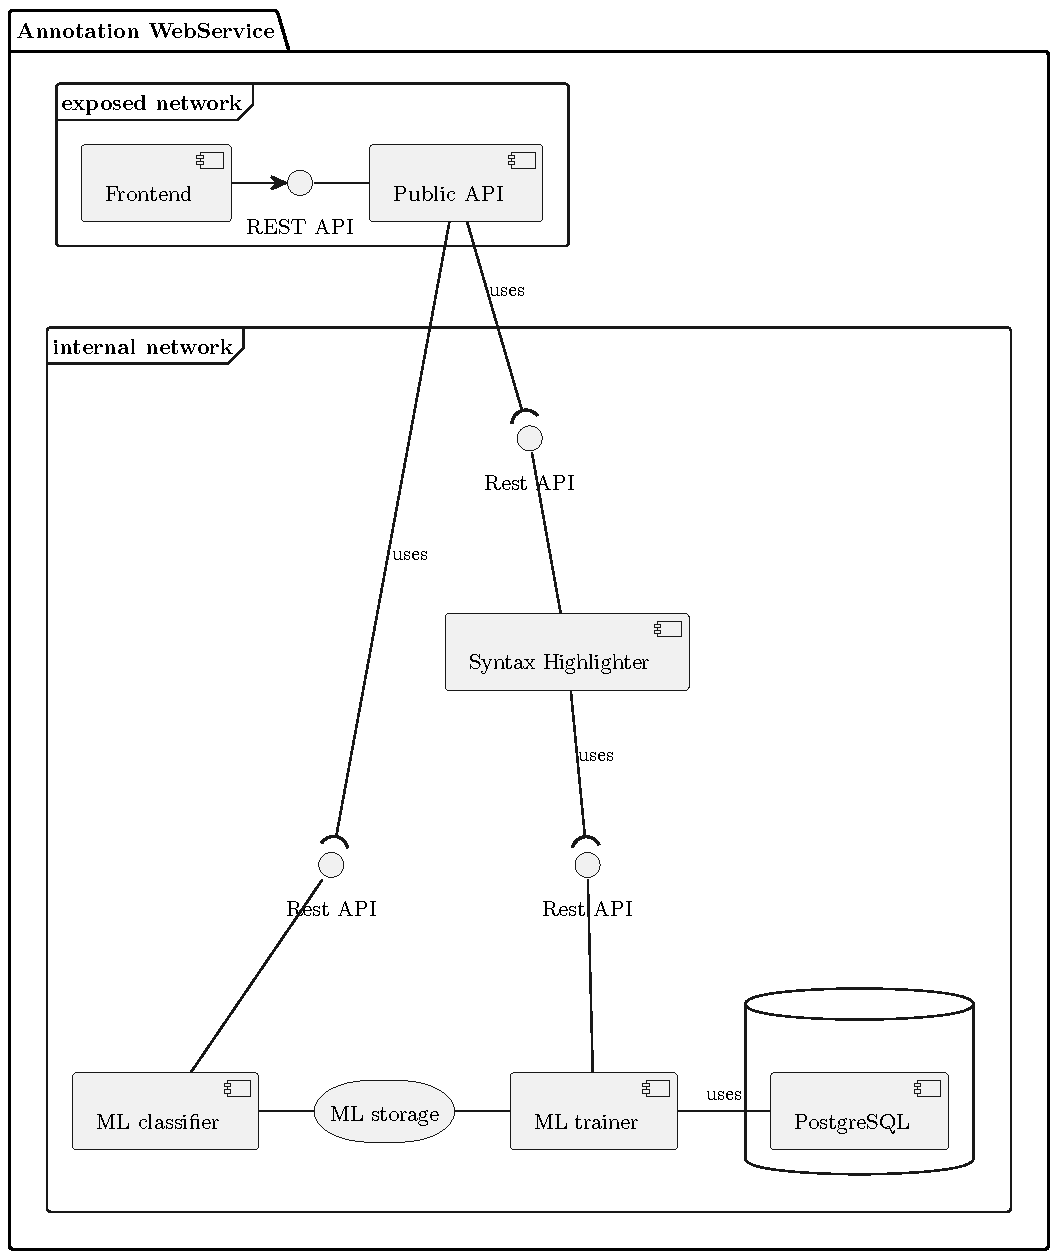
\includegraphics[width=0.5\linewidth]{illustations/architecture.pdf}
    \caption{Microservice architecture}
    \label{fig:uml_architecture}
\end{figure}

We are going to use microservice architecture. A microservice architecture makes sense in our case, as we have different parts of our system that are written using different technologies. An overview of our microservice architecture can be seen in Figure \ref{fig:uml_architecture}. Every single component in our architecture is a single running \textit{Docker} container. Using \textit{Docker Compose}, we will link them all together. This allows us to have two separate networks, one that is accessible from outside including the GUI and our public API and one that is only used internally by \textit{Docker Compose}.

\begin{figure}
    \centering
    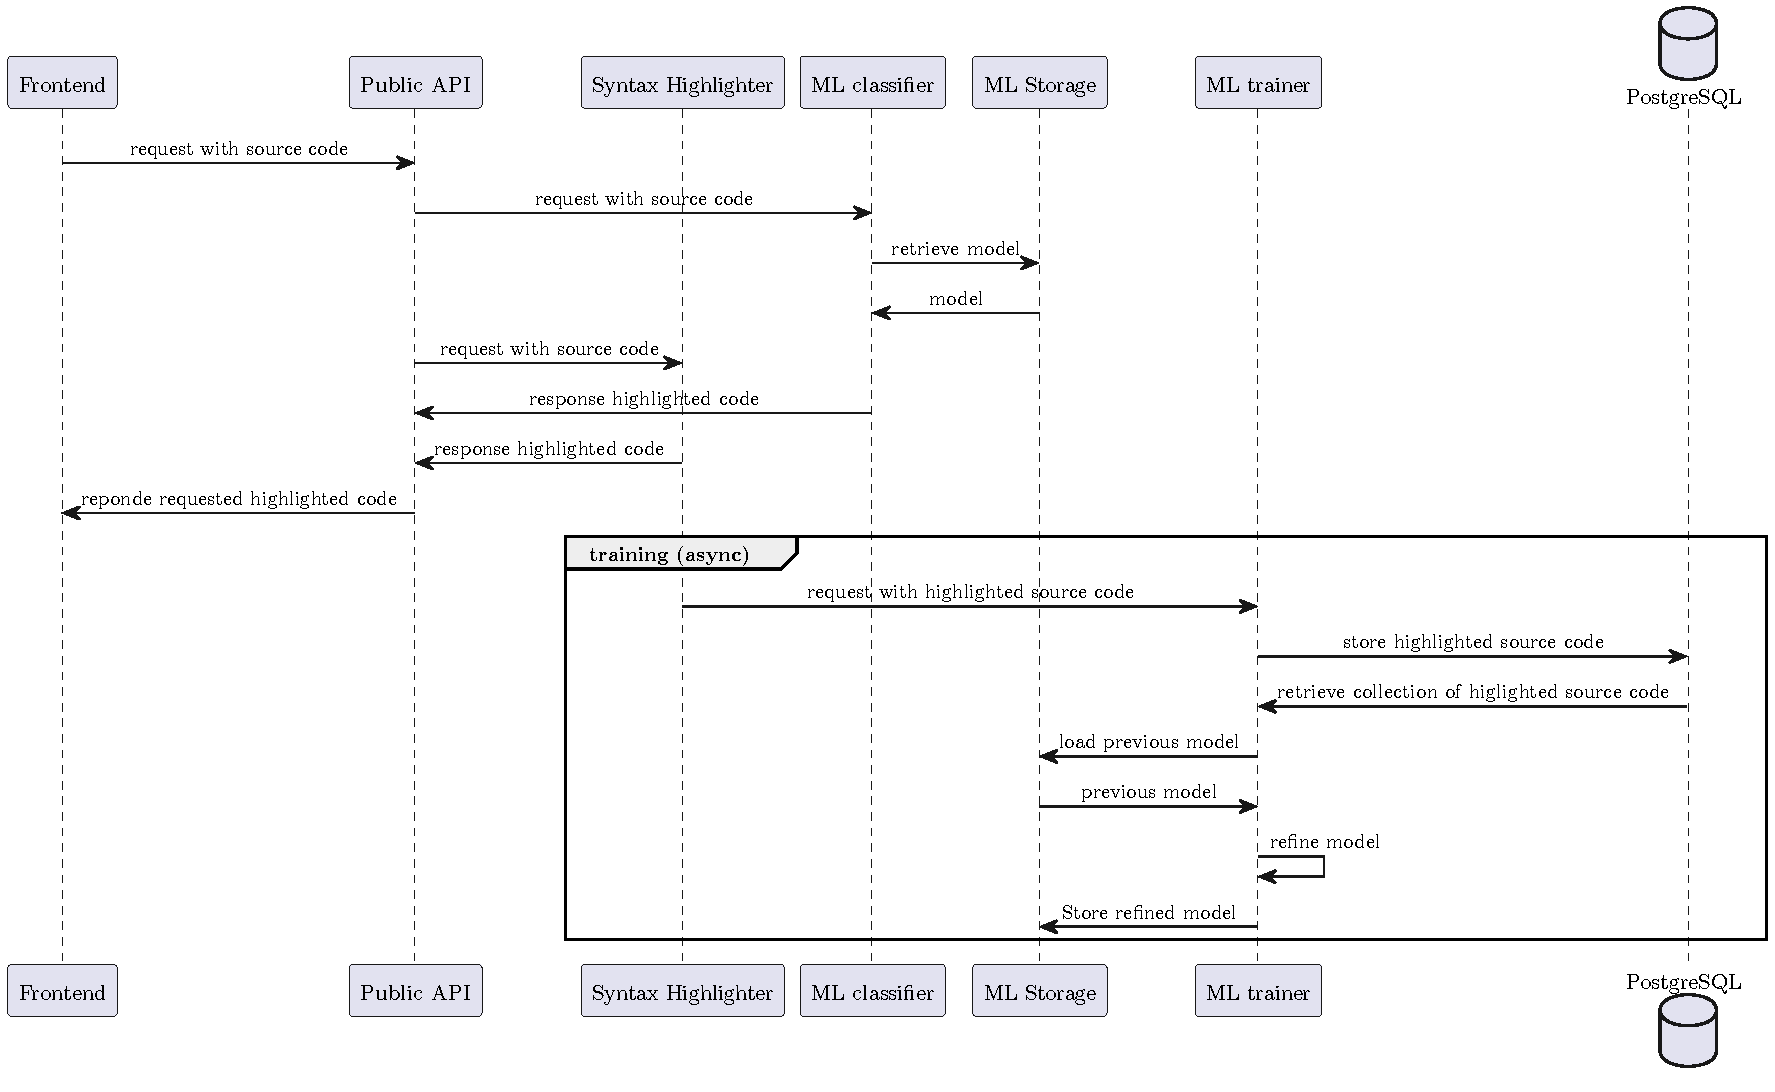
\includegraphics[width=\linewidth]{illustations/sequence.pdf}
    \caption{Sequence of a request and the training}
    \label{fig:uml_sequence}
\end{figure}

Whenever possible and convenient, the different services of our architecture will communicate with each other through well-defined \texttt{REST APIs}. The two exceptions to this are the shared model storage and the database. The reasons for deviating from \texttt{REST APIs} are the following: For the model storage, it doesn't make sense to use a \texttt{REST API} as the learner provided\footnote{\url{https://github.com/MEPalma/UZH-ASE-AnnotationWS-BaseLearner}} is based on a file, as such it would not make sense to share the model through an API and using a file storage ensures both the learner and classifier have the same model available to them. Secondly, for the database it doesn't make sense to write an additional interface in front of the database, as database interfaces are widely available for almost all languages and take away a lot of the complexity. Figure \ref{fig:uml_sequence} shows the sequence of requests and the internal communication.

We use Java for the \textit{Syntax Highlighter}, as the base project is written in Java. For the \textit{ML trainer} and the \textit{ML classifier}, we use Python for the same reason, building a lightweight Flask frontend that provides the API. For the database we are going to use \textit{PostgreSQL} as it is widely used and has great libraries to use in Python. For the \textit{Public API} we are going to use a simple \textit{Node.js/Express} server as this component doesn't need to do much. Finally, the frontend will be written in react or angular. We are not 100\% sure which of the frameworks we are going to use, as this depends a lot on which developer is going to perform that task.

\end{document}